\chapter{O metabolismo celular}\label{ch:g10:cell-metabolism}

Estique uma bexiga sobre o gargalo de um frasco com água açucarada
morna e uma colherada de fermento biológico dentro. Em menos de uma
hora o líquido fica turvo e efervescente, a bexiga se levanta e o
frasco cheira de leve a pão e a cerveja. As \omterm{def:g10:cells-common-unit:cell}{células} de levedura estão
comendo o açúcar e o transformando em outra coisa, e o gás que elas
liberam é o mesmo gás carbônico que você expira. Uma folha ao sol faz o
contrário: capta gás carbônico e libera oxigênio. Os dois casos são
química, feita dentro de \omterm{def:g10:cells-common-unit:cell}{células}, à temperatura do corpo, sem chama e
sem ácido --- e este capítulo trata dessa química.

\section{O metabolismo: a química de uma célula}

\begin{definition}[Metabolismo]\label{def:g10:cell-metabolism:metabolism}
O \emph{metabolismo}\index{metabolismo} de uma \omterm{def:g10:cells-common-unit:cell}{célula} é o conjunto de
todas as reações químicas que acontecem dentro dela: as que degradam
moléculas para liberar energia e as que constroem as moléculas próprias
da \omterm{def:g10:cells-common-unit:cell}{célula} a partir de outras mais simples. Toda reação do metabolismo é
conduzida por uma \emph{enzima}\index{enzima}, uma \omterm{def:g10:chemistry-of-life:families}{proteína} que acelera
uma reação específica sem ser consumida por ela.
\end{definition}

\begin{proposition}[As enzimas tornam possível a química da célula]\label{prop:g10:cell-metabolism:enzymes}
A glicose deixada ao ar a \qty{37}{\celsius} não queima; numa \omterm{def:g10:cells-common-unit:cell}{célula}
ela é oxidada por completo em poucos minutos. A diferença são as
\omterm{def:g10:cell-metabolism:metabolism}{enzimas}: cada uma se liga a uma molécula particular (o
\emph{substrato} dela), a transforma num produto, o libera e recomeça,
milhares de vezes por segundo. O \omterm{def:g10:cell-metabolism:metabolism}{metabolismo} de uma \omterm{def:g10:cells-common-unit:cell}{célula} é fixado,
portanto, pelo conjunto de \omterm{def:g10:cell-metabolism:metabolism}{enzimas} que ela possui --- e esse conjunto é
fixado pelos \omterm{def:g10:universal-dna:gene}{genes} dela.
\end{proposition}
\admitted

\begin{example}[Uma enzima em ação]\label{ex:g10:cell-metabolism:catalase}
Despeje água oxigenada sobre um pedaço de fígado cru ou de batata: ela
espuma violentamente à medida que o oxigênio é liberado. A \omterm{def:g10:cell-metabolism:metabolism}{enzima}
catalase, presente em quase toda \omterm{def:g10:cells-common-unit:cell}{célula}, quebra o peróxido tóxico em
água e oxigênio a uma taxa de milhões de moléculas por segundo por
molécula de \omterm{def:g10:cell-metabolism:metabolism}{enzima}. Ferva o fígado antes e nada acontece: a \omterm{def:g10:cell-metabolism:metabolism}{enzima}, uma
\omterm{def:g10:chemistry-of-life:families}{proteína}, foi destruída pelo calor. A água oxigenada sem borbulhar
sobre uma pedra mostra que a reação não corre sozinha.
\end{example}

\begin{omfigure}
\begin{tikzpicture}[>=Stealth, font=\small]
  \node[draw, rounded corners, fill=omDef!15, minimum width=1.6cm, minimum height=1.1cm] (e1) at (0,0) {enzima};
  \node[draw, fill=omProp!30, minimum width=0.9cm, minimum height=0.5cm] (s) at (0,1.3) {substrato};
  \draw[->] (s) -- (e1);
  \node[draw, rounded corners, fill=omDef!15, minimum width=1.6cm, minimum height=1.1cm] (e2) at (4,0) {enzima};
  \node[draw, fill=omProp!30, minimum width=0.9cm, minimum height=0.5cm, anchor=south] (s2) at (4,0.55) {substrato};
  \draw[->] (e1.east) -- node[above] {liga-se} (e2.west);
  \node[draw, rounded corners, fill=omDef!15, minimum width=1.6cm, minimum height=1.1cm] (e3) at (8,0) {enzima};
  \node[draw, fill=omMeth!30, minimum width=0.5cm, minimum height=0.5cm] (p1) at (7.5,1.5) {produto};
  \node[draw, fill=omMeth!30, minimum width=0.5cm, minimum height=0.5cm] (p2) at (9.1,1.5) {produto};
  \draw[->] (e2.east) -- node[above] {transforma} (e3.west);
  \draw[->] (e3.north) -- (p1.south);
  \draw[->] (e3.north) -- (p2.south);
  \draw[->, dashed] (e3.south) to[bend left=25] node[below] {liberada intacta, recomeça} (e1.south);
\end{tikzpicture}

{\small Uma \omterm{def:g10:cell-metabolism:metabolism}{enzima} se liga ao substrato dela, o transforma e libera o
produto, permanecendo ela mesma intacta. Uma molécula de \omterm{def:g10:cell-metabolism:metabolism}{enzima} pode
repetir o ciclo milhares de vezes por segundo.}
\end{omfigure}

\section{Dois modos de alimentar uma célula}

\begin{definition}[Autotrofia e heterotrofia]\label{def:g10:cell-metabolism:autotrophy}
Uma \omterm{def:g10:cells-common-unit:cell}{célula} é \emph{autotrófica}\index{autotrofia} se constrói as
moléculas orgânicas próprias a partir de \omterm{def:g10:chemistry-of-life:mineral-organic}{matéria mineral} apenas ---
gás carbônico, água, \omterm{def:g10:chemistry-of-life:mineral-organic}{sais minerais} ---, usando uma fonte externa de
energia. As \omterm{def:g10:cells-common-unit:cell}{células} vegetais com \omterm{def:g10:cells-common-unit:organelle}{cloroplastos}, as algas e algumas
bactérias são autótrofas, e a fonte de energia delas é a luz: é a
\emph{fotossíntese}\index{fotossíntese}. Uma \omterm{def:g10:cells-common-unit:cell}{célula} é
\emph{heterotrófica}\index{heterotrofia} se precisa captar moléculas
orgânicas fabricadas por outros organismos, tanto como material de
construção quanto como fonte de energia: as \omterm{def:g10:cells-common-unit:cell}{células} animais, os fungos,
a maioria das bactérias e as \omterm{def:g10:cells-common-unit:cell}{células} não verdes dos vegetais (as
raízes, por exemplo) são heterótrofas.
\end{definition}

\begin{proposition}[A fotossíntese]\label{prop:g10:cell-metabolism:photosynthesis}
Na luz, uma \omterm{def:g10:cells-common-unit:cell}{célula} que contém \omterm{def:g10:cells-common-unit:organelle}{cloroplastos} absorve gás carbônico e
água, libera oxigênio e constrói glicose, que ela converte em seguida
em amido, celulose, \omterm{def:g10:chemistry-of-life:families}{lipídios} e, com nitrogênio mineral, \omterm{def:g10:chemistry-of-life:families}{aminoácidos}.
Em resumo:
\[
6\,\mathrm{CO_2} + 6\,\mathrm{H_2O} \xrightarrow{\ \text{luz, clorofila}\ }
\mathrm{C_6H_{12}O_6} + 6\,\mathrm{O_2}.
\]
A energia da luz fica armazenada nas ligações químicas da glicose.
\end{proposition}
\begin{proof}[Evidências]
Uma suspensão da alga verde \emph{Chlorella} num recipiente fechado
equipado com uma sonda de oxigênio mostra o oxigênio dissolvido subindo
com regularidade quando a lâmpada está acesa e caindo quando ela está
apagada; a subida cessa se o gás carbônico da água for retirado. Folhas
mantidas no escuro por dois dias não coram mais de azul-escuro com o
iodo, e uma folha coberta pela metade com papel-alumínio cora só na
metade exposta: o amido é fabricado onde a luz incide. Gás carbônico
radioativo fornecido a uma planta vai parar nos açúcares dela em poucos
minutos.
\end{proof}

\begin{omfigure}
\begin{tikzpicture}
\begin{axis}[
  width=0.88\linewidth, height=5.4cm,
  axis x line=bottom, axis y line=left,
  xmin=0, xmax=22, ymin=5, ymax=13,
  xlabel={tempo (min)}, ylabel={$\mathrm{O_2}$ dissolvido (mg/L)},
  xlabel style={font=\small, at={(axis description cs:0.5,-0.12)}, anchor=north},
  ylabel style={font=\small},
  tick label style={font=\small}, xtick={0,5,10,15,20},
  clip=false,
]
\addplot[thick, omMeth] coordinates {(0,8.0) (5,8.0) (10,10.5) (15,10.0) (20,12.5)};
\draw[dashed, gray] (axis cs:5,5) -- (axis cs:5,13);
\draw[dashed, gray] (axis cs:10,5) -- (axis cs:10,13);
\draw[dashed, gray] (axis cs:15,5) -- (axis cs:15,13);
\node[font=\small, anchor=south] at (axis cs:2.5,12.5) {escuro};
\node[font=\small, anchor=south] at (axis cs:7.5,12.5) {luz};
\node[font=\small, anchor=south] at (axis cs:12.5,12.5) {escuro};
\node[font=\small, anchor=south] at (axis cs:17.5,12.5) {luz};
\end{axis}
\end{tikzpicture}

{\small Oxigênio dissolvido numa suspensão fechada de \emph{Chlorella}.
Na luz as algas liberam oxigênio mais depressa do que o consomem; no
escuro resta apenas a respiração delas e o oxigênio cai. Cada
inclinação é uma taxa, legível em miligramas por litro por minuto.}
\end{omfigure}

\begin{example}[A euglena, as duas coisas ao mesmo tempo]\label{ex:g10:cell-metabolism:euglena}
A \emph{Euglena}, unicelular, tem \omterm{def:g10:cells-common-unit:organelle}{cloroplastos} e nada com um flagelo.
Na luz, em água mineral, ela cresce: autótrofa. No escuro, ela só
sobrevive se moléculas orgânicas forem acrescentadas à água, e ela as
absorve: heterótrofa. Mantida muito tempo no escuro, ela perde os
\omterm{def:g10:cells-common-unit:organelle}{cloroplastos}; devolvida à luz, com alguns dias de paciência, ela os
fabrica de novo. O \omterm{def:g10:cell-metabolism:metabolism}{metabolismo} dela depende dos \omterm{def:g10:universal-dna:gene}{genes} dela, que
permitem as duas opções, e do ambiente dela, que seleciona uma.
\end{example}

\section{Obter energia das moléculas orgânicas}

\begin{proposition}[A respiração celular]\label{prop:g10:cell-metabolism:respiration}
Toda \omterm{def:g10:cells-common-unit:cell}{célula}, autótrofa ou heterótrofa, obtém energia utilizável
degradando moléculas orgânicas. Quando há oxigênio disponível, a
degradação é completa --- é a \emph{respiração celular}\index{respiração celular},
nas \omterm{def:g10:cells-common-unit:organelle}{mitocôndrias}:
\[
\mathrm{C_6H_{12}O_6} + 6\,\mathrm{O_2} \longrightarrow
6\,\mathrm{CO_2} + 6\,\mathrm{H_2O} + \text{energia},
\]
cerca de \qty{2870}{kJ} por mol de glicose (\qty{180}{g}), dos quais
aproximadamente 40\% são capturados numa molécula pequena, o
\emph{ATP}\index{ATP}, de que todo processo da \omterm{def:g10:cells-common-unit:cell}{célula} que exige energia
--- movimento, transporte, síntese --- lança mão; o resto é liberado
como calor.
\end{proposition}
\begin{proof}[Evidências]
Uma levedura num recipiente fechado com uma sonda de oxigênio não
consome oxigênio nenhum enquanto está em jejum; acrescente glicose e o
oxigênio dissolvido cai a uma taxa constante enquanto gás carbônico
aparece, até o oxigênio se esgotar. Sementes em germinação numa garrafa
térmica aquecem a garrafa em vários graus em um dia --- o calor da
respiração ---, enquanto sementes fervidas não. As \omterm{def:g10:cells-common-unit:cell}{células} musculares
vistas ao microscópio eletrônico estão abarrotadas de \omterm{def:g10:cells-common-unit:organelle}{mitocôndrias}, e
um veneno das \omterm{def:g10:cells-common-unit:organelle}{mitocôndrias} faz o músculo parar.
\end{proof}

\begin{omfigure}
\begin{tikzpicture}
\begin{axis}[
  width=0.88\linewidth, height=5.4cm,
  axis x line=bottom, axis y line=left,
  xmin=0, xmax=12, ymin=0, ymax=10,
  xlabel={tempo (min)}, ylabel={$\mathrm{O_2}$ dissolvido (mg/L)},
  xlabel style={font=\small, at={(axis description cs:0.5,-0.12)}, anchor=north},
  ylabel style={font=\small},
  tick label style={font=\small}, xtick={0,2,4,6,8,10,12},
  clip=false,
]
\addplot[thick, omThm] coordinates {(0,8.0) (3,7.9) (10,0.9) (12,0.6)};
\draw[->, thick] (axis cs:3,9.6) -- (axis cs:3,8.3);
\node[font=\small, anchor=south] at (axis cs:3,9.7) {glicose acrescentada};
\end{axis}
\end{tikzpicture}

{\small Oxigênio dissolvido numa suspensão fechada de levedura. A
levedura em jejum quase não consome nada; assim que a glicose é
acrescentada, o oxigênio cai a \qty{1.0}{mg/L} por minuto --- a taxa da
respiração --- até acabar.}
\end{omfigure}

\begin{definition}[Fermentação]\label{def:g10:cell-metabolism:fermentation}
Sem oxigênio, algumas \omterm{def:g10:cells-common-unit:cell}{células} degradam a glicose apenas parcialmente,
no \omterm{def:g10:cells-common-unit:cell}{citoplasma}, em moléculas orgânicas menores que ainda guardam a maior
parte da energia: é a \emph{fermentação}\index{fermentação}. A levedura
faz a fermentação alcoólica,
\[
\mathrm{C_6H_{12}O_6} \longrightarrow 2\,\mathrm{C_2H_5OH} +
2\,\mathrm{CO_2} + \text{energia},
\]
e as \omterm{def:g10:cells-common-unit:cell}{células} musculares com falta de oxigênio, assim como as bactérias
do iogurte, fazem a fermentação láctica, transformando a glicose em
ácido láctico. Uma fermentação rende cerca de quinze vezes menos ATP
por glicose do que a respiração.
\end{definition}

\begin{omfigure}
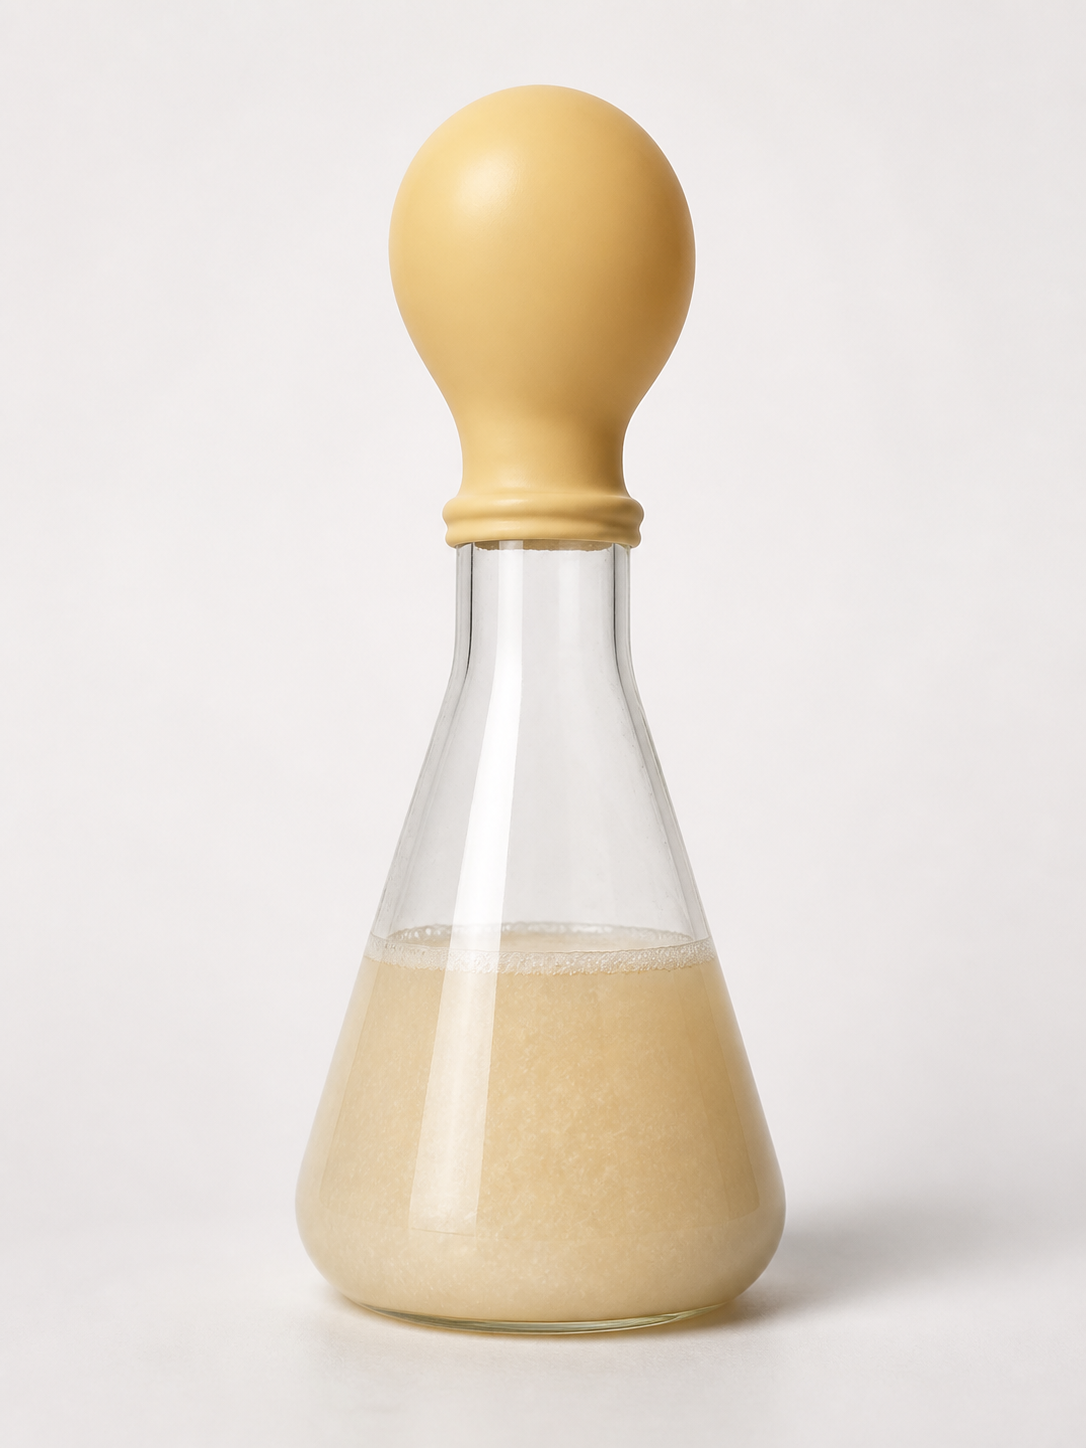
\includegraphics[width=0.36\linewidth]{images/book2/ai/g10-metab-yeast-balloon.png}

{\small Levedura fermentando açúcar num frasco: o gás carbônico da
\omterm{def:g10:cell-metabolism:fermentation}{fermentação} alcoólica infla a bexiga. Sem oxigênio no líquido, o açúcar
é degradado apenas em parte e o etanol fica para trás.}
\end{omfigure}

\begin{example}[A levedura no ar e fora dele]\label{ex:g10:cell-metabolism:pasteur}
A levedura borbulhada com ar usa a glicose com parcimônia e cresce
depressa: ela respira. A mesma levedura numa cuba fechada usa a glicose
com voracidade, cresce pouco e fabrica etanol: ela fermenta. Pasteur,
que descreveu isso em 1861, chamou a \omterm{def:g10:cell-metabolism:fermentation}{fermentação} de ``vida sem ar''; as
\omterm{def:g10:cells-common-unit:cell}{células} mudam o \omterm{def:g10:cell-metabolism:metabolism}{metabolismo} delas para a via que o ambiente permitir e,
como a \omterm{def:g10:cell-metabolism:fermentation}{fermentação} dá tão pouca energia por glicose, elas precisam
queimar muito mais açúcar para viver.
\end{example}

\begin{omfigure}
\begin{tikzpicture}[>=Stealth, font=\small,
  cell/.style={draw, rounded corners, thick, minimum height=1.5cm, text width=2.7cm, align=center},
  inp/.style={text width=2.3cm, align=right, anchor=east},
  outp/.style={text width=2.6cm, align=left, anchor=west}]
  \node[cell, fill=omMeth!12] (a) at (0,0) {\textbf{célula autótrofa}\\ cloroplastos};
  \node[inp] (ai) at (-2.2,0) {$\mathrm{CO_2}$, $\mathrm{H_2O}$,\\ sais minerais,\\ \emph{luz}};
  \node[outp] (ao) at (2.2,0) {matéria orgânica\\ (glicose, amido\dots)\\ $+ \mathrm{O_2}$};
  \draw[->] (ai) -- (a); \draw[->] (a) -- (ao);
  \node[cell, fill=omThm!10] (h) at (0,-3.2) {\textbf{qualquer célula}\\ mitocôndrias};
  \node[inp] (hi) at (-2.2,-3.2) {matéria orgânica\\ $+ \mathrm{O_2}$};
  \node[outp] (ho) at (2.2,-3.2) {$\mathrm{CO_2}$, $\mathrm{H_2O}$\\ $+$ energia (ATP, calor)};
  \draw[->] (hi) -- (h); \draw[->] (h) -- (ho);
  \node[anchor=west, font=\small\itshape] at (8.6,0) {fotossíntese};
  \node[anchor=west, font=\small\itshape] at (8.6,-3.2) {respiração};
  \draw[->, gray, thick] (4.6,-0.7) to[bend left=35] node[right, font=\scriptsize, text width=3.6cm, align=left, xshift=2pt] {a matéria orgânica alimenta os heterótrofos, e a própria respiração do autótrofo} (4.6,-2.5);
\end{tikzpicture}

{\small Os dois fluxos do \omterm{def:g10:cell-metabolism:metabolism}{metabolismo} celular. A \omterm{def:g10:cell-metabolism:autotrophy}{fotossíntese} armazena
energia luminosa em \omterm{def:g10:chemistry-of-life:mineral-organic}{matéria orgânica}; a respiração, em toda \omterm{def:g10:cells-common-unit:cell}{célula}, a
libera. Os autótrofos fazem as duas coisas; os heterótrofos fazem só a
segunda e precisam ser alimentados com \omterm{def:g10:chemistry-of-life:mineral-organic}{matéria orgânica}.}
\end{omfigure}

\section{O que decide o metabolismo de uma célula}

\begin{proposition}[Genes e ambiente]\label{prop:g10:cell-metabolism:decides}
O \omterm{def:g10:cell-metabolism:metabolism}{metabolismo} de uma \omterm{def:g10:cells-common-unit:cell}{célula} depende de duas coisas: do
\emph{equipamento} dela --- as \omterm{def:g10:cell-metabolism:metabolism}{enzimas} e as \omterm{def:g10:cells-common-unit:organelle}{organelas} que os \omterm{def:g10:universal-dna:gene}{genes}
dela permitem construir, de modo que uma \omterm{def:g10:cells-common-unit:cell}{célula} sem clorofila jamais
poderá fazer \omterm{def:g10:cell-metabolism:autotrophy}{fotossíntese} --- e do \emph{ambiente} dela --- luz,
oxigênio, nutrientes disponíveis ---, que decide qual das vias
possíveis efetivamente funciona. Uma levedura é respiradora no ar e
fermentadora sem ele; uma \emph{Euglena} é autótrofa na luz e
heterótrofa no escuro; uma \omterm{def:g10:cells-common-unit:cell}{célula} de raiz de uma planta verde é
heterótrofa a vida inteira, alimentada pelas folhas.
\end{proposition}
\admitted

\begin{method}[Ler um traçado metabólico]\label{met:g10:cell-metabolism:trace}
Os experimentos com sonda de oxigênio dão uma concentração em função do
tempo.
\begin{enumerate}
  \item Identifique o que mudou em cada instante marcado (luz acesa,
        substrato acrescentado, oxigênio esgotado).
  \item Leia a inclinação de cada trecho retilíneo: variação vertical
        sobre variação horizontal, em \unit{mg/L} por minuto. Uma
        inclinação positiva significa produção líquida de oxigênio;
        uma negativa, consumo líquido.
  \item Lembre que uma \omterm{def:g10:cells-common-unit:cell}{célula} que faz \omterm{def:g10:cell-metabolism:autotrophy}{fotossíntese} também respira: a
        inclinação na luz é a produção menos a respiração, de modo que
        a taxa verdadeira de \omterm{def:g10:cell-metabolism:autotrophy}{fotossíntese} é a inclinação na luz mais o
        tamanho da inclinação no escuro.
  \item Converta se for pedido: nessas concentrações, \qty{1}{mg/L} de
        oxigênio dissolvido é $1/32$ de milimol por litro.
\end{enumerate}
\end{method}

\begin{example}[A taxa verdadeira da alga]\label{ex:g10:cell-metabolism:truerate}
Na figura da \emph{Chlorella} o oxigênio sobe \qty{2.5}{mg/L} em 5
minutos de luz (inclinação $+0.5$) e cai \qty{0.5}{mg/L} em 5 minutos
de escuro (inclinação $-0.1$). A respiração consome \qty{0.1}{mg/L} por
minuto também na luz, de modo que a \omterm{def:g10:cell-metabolism:autotrophy}{fotossíntese} produz
$0.5 + 0.1 = \qty{0.6}{mg/L}$ por minuto: seis vezes o que a respiração
usa. A alga é produtora líquida de oxigênio e de \omterm{def:g10:chemistry-of-life:mineral-organic}{matéria orgânica}, e é
por isso que ela cresce.
\end{example}

\section{Exercícios}

\begin{exercise}[$\star$]\label{exo:g10:cell-metabolism:1}
Defina \omterm{def:g10:cell-metabolism:metabolism}{metabolismo}, e diga o que é uma \omterm{def:g10:cell-metabolism:metabolism}{enzima} e o que ela faz.
\end{exercise}

\begin{exercise}[$\star$]\label{exo:g10:cell-metabolism:2}
Escreva a equação-resumo da \omterm{prop:g10:cell-metabolism:respiration}{respiração celular} e a da \omterm{def:g10:cell-metabolism:autotrophy}{fotossíntese}. Em
que sentido uma é o inverso da outra, e em que sentido não é?
\end{exercise}

\begin{exercise}[$\star$]\label{exo:g10:cell-metabolism:3}
Classifique como autótrofo ou heterótrofo: um cogumelo, um musgo, uma
\omterm{def:g10:cells-common-unit:cell}{célula} de raiz de cenoura, uma clorela, uma bactéria do iogurte, uma
\omterm{def:g10:cells-common-unit:cell}{célula} muscular humana.
\end{exercise}

\begin{exercise}[$\star$]\label{exo:g10:cell-metabolism:4}
No experimento da levedura com a bexiga, que gás infla a bexiga, que
produto líquido se acumula, e o que falta ao frasco que mudaria o
resultado?
\end{exercise}

\begin{exercise}[$\star$]\label{exo:g10:cell-metabolism:5}
Por que o fígado fervido não faz mais a água oxigenada espumar?
\end{exercise}

\begin{exercise}[$\star\star$]\label{exo:g10:cell-metabolism:6}
Na figura da levedura, o oxigênio cai de \qty{7.9}{mg/L} para
\qty{0.9}{mg/L} entre os minutos 3 e 10. Calcule a taxa de respiração
em \unit{mg/L} por minuto. Por que a curva se achata depois do minuto
10, e o que a levedura faz então?
\end{exercise}

\begin{exercise}[$\star\star$]\label{exo:g10:cell-metabolism:7}
Uma clorela na luz apresenta uma inclinação de oxigênio de $+0.8$
\unit{mg/L} por minuto e, no escuro, de $-0.2$. Calcule a taxa de
\omterm{def:g10:cell-metabolism:autotrophy}{fotossíntese}.
\end{exercise}

\begin{exercise}[$\star\star$]\label{exo:g10:cell-metabolism:8}
Uma \omterm{def:g10:cells-common-unit:cell}{célula} respira \qty{18}{g} de glicose. Que massa de oxigênio ela
usa e que massa de gás carbônico ela libera? (Massas molares: glicose
\qty{180}{g/mol}, $\mathrm{O_2}$ \qty{32}{g/mol},
$\mathrm{CO_2}$ \qty{44}{g/mol}.)
\end{exercise}

\begin{exercise}[$\star\star$]\label{exo:g10:cell-metabolism:9}
Ervilhas em germinação numa garrafa térmica elevam a temperatura dela
em \qty{4}{\celsius} em um dia; ervilhas fervidas não. Explique os dois
resultados, e diga por que a garrafa não pode ficar hermeticamente
fechada.
\end{exercise}

\begin{exercise}[$\star\star$]\label{exo:g10:cell-metabolism:10}
Uma folha verde é mantida no escuro por 48 horas, depois metade dela é
coberta com papel preto e a planta é posta ao sol por um dia. Aplica-se
iodo. Preveja e explique o resultado em cada metade, e diga por que as
48 horas de escuro foram necessárias.
\end{exercise}

\begin{exercise}[$\star\star$]\label{exo:g10:cell-metabolism:11}
Explique por que a levedura numa cuba fechada consome açúcar muito mais
depressa, por \omterm{def:g10:cells-common-unit:cell}{célula}, que a levedura borbulhada com ar.
\end{exercise}

\begin{exercise}[$\star\star\star$]\label{exo:g10:cell-metabolism:12}
Os músculos de um velocista ficam doloridos e ácidos depois de uma
corrida de 400 metros. Explique o que aconteceu nas \omterm{def:g10:cells-common-unit:cell}{células} musculares,
por que aconteceu, e por que os músculos do mesmo corredor não ficam
ácidos durante um trote leve.
\end{exercise}

\begin{exercise}[$\star\star\star$]\label{exo:g10:cell-metabolism:13}
Uma \emph{Euglena} mantida um mês no escuro com alimento orgânico perde
os \omterm{def:g10:cells-common-unit:organelle}{cloroplastos}, mas os descendentes dela os recuperam na luz. Qual dos
dois fatores da \cref{prop:g10:cell-metabolism:decides} mudou e qual
não mudou? O que a recuperação prova a respeito dos \omterm{def:g10:universal-dna:gene}{genes} da \omterm{def:g10:cells-common-unit:cell}{célula}?
\end{exercise}

\begin{exercise}[$\star\star\star$]\label{exo:g10:cell-metabolism:14}
Um aquário fechado contém água, um caramujo e uma planta aquática, na
luz. Explique como os dois organismos podem sobreviver meses, o que
cada um fornece ao outro, e o que acontece se o aquário for mantido no
escuro.
\end{exercise}

\begin{exercise}[$\star\star\star$]\label{exo:g10:cell-metabolism:15}
A respiração de uma glicose rende cerca de 30 ATP, a \omterm{def:g10:cell-metabolism:fermentation}{fermentação} 2. Uma
\omterm{def:g10:cells-common-unit:cell}{célula} de levedura precisa de um número fixo de ATP por minuto para
viver. Calcule quantas vezes mais glicose ela precisa consumir por
minuto quando fermenta; depois explique por que os cervejeiros mantêm o
ar longe das cubas deles mesmo que isso ``desperdice'' açúcar.
\end{exercise}

\section{Problema: a cuba do vinicultor}

\begin{problem}[{Problema de fim de semana --- uma cuba de suco de uva
entregue à levedura: o álcool que ela vai conter, o gás que ela vai
liberar, o calor que ela vai produzir, e por que uma adega pode ser um
lugar perigoso}]
\label{pb:g10:cell-metabolism:1}
O suco de uva (o mosto) contém cerca de \qty{200}{g} de açúcar por
litro, que tomamos como glicose, e nenhum oxigênio dissolvido depois de
a cuba ser fechada. Massas molares: glicose \qty{180}{g/mol}, etanol
$\mathrm{C_2H_5OH}$ \qty{46}{g/mol}, gás carbônico \qty{44}{g/mol},
oxigênio \qty{32}{g/mol}. A densidade do etanol é \qty{0.79}{g/mL}. Um
mol de gás ocupa cerca de \qty{24}{L} à temperatura da adega. A cuba
comporta \qty{1000}{L}.

\medskip
\noindent\textbf{Parte I --- O que a levedura fabrica.}
\begin{enumerate}
  \item Que via a levedura usa na cuba fechada, e por quê? Escreva a
        equação dela.
  \item Quantos mols de glicose contém um litro de mosto?
  \item Calcule a massa de etanol produzida por litro, depois o volume
        dele, depois o teor alcoólico do vinho em por cento em volume.
  \item Calcule a massa de gás carbônico produzida por litro de mosto,
        e o volume dela como gás.
  \item Para a cuba inteira, que volume de gás carbônico é liberado?
        Compare com o volume de uma adega de \qty{4}{m} por \qty{6}{m}
        por \qty{2.5}{m}.
\end{enumerate}

\medskip
\noindent\textbf{Parte II --- Se a levedura tivesse ar.}
\begin{enumerate}[resume]
  \item Escreva a equação que a levedura seguiria se o mosto fosse
        continuamente aerado.
  \item Calcule a massa de oxigênio necessária para respirar o açúcar
        de um litro de mosto, e a massa de gás carbônico liberada.
  \item Compare o gás carbônico da questão 7 com o da questão 4, e
        explique a diferença em termos de até onde a glicose é
        degradada.
  \item A respiração rende cerca de 30 ATP por glicose e a \omterm{def:g10:cell-metabolism:fermentation}{fermentação}
        2. Se a levedura precisa do mesmo ATP nos dois casos, em qual
        deles o açúcar dura mais, e por que fator?
  \item Explique por que, apesar disso, um vinicultor mantém o ar longe.
\end{enumerate}

\medskip
\noindent\textbf{Parte III --- O calor da cuba.}
A \omterm{def:g10:cell-metabolism:fermentation}{fermentação} libera cerca de \qty{70}{kJ} de calor por mol de glicose;
aquecer \qty{1}{kg} de água em \qty{1}{\celsius} exige \qty{4.2}{kJ}.
\begin{enumerate}[resume]
  \item Calcule o calor liberado por litro de mosto, depois para a
        cuba.
  \item Se nada dele escapasse, de quanto subiria a temperatura da
        cuba? (Tome o mosto como água.)
  \item As \omterm{def:g10:cell-metabolism:metabolism}{enzimas} da levedura são destruídas acima de cerca de
        \qty{40}{\celsius}. Partindo de \qty{20}{\celsius}, uma cuba
        sem refrigeração sobreviveria? O que isso diz a você sobre por
        que as cubas grandes são refrigeradas?
  \item Explique, usando a \cref{prop:g10:cell-metabolism:enzymes}, por
        que o calor interrompe a \omterm{def:g10:cell-metabolism:fermentation}{fermentação} mesmo com o açúcar ainda
        presente.
  \item A respiração teria liberado cerca de \qty{2870}{kJ} por mol.
        Onde permanece a energia que a \omterm{def:g10:cell-metabolism:fermentation}{fermentação} \emph{não} libera?
\end{enumerate}

\medskip
\noindent\textbf{Parte IV --- A adega.}
\begin{enumerate}[resume]
  \item O gás carbônico é mais denso que o ar. Onde ele se acumula na
        adega, e por que uma vela acesa levada rente ao chão é um teste
        tradicional de segurança?
  \item As \omterm{def:g10:cells-common-unit:cell}{células} de um trabalhador, privadas de oxigênio, passariam a
        que via --- e por que um corpo humano não consegue viver dela
        por mais do que alguns minutos?
  \item A \omterm{def:g10:cell-metabolism:fermentation}{fermentação} para sozinha quando o álcool chega a cerca de
        15\% em volume. Proponha uma explicação em termos das \omterm{def:g10:cell-metabolism:metabolism}{enzimas}
        da levedura.
  \item A massa de pão usa a mesma levedura por uma hora. O que contêm
        as bolhas do miolo, e para onde foi o etanol depois de assado?
  \item Enuncie o resultado: para um litro de mosto, o teor alcoólico e
        o volume de gás produzido --- e o único fato metabólico que
        explica os dois.
\end{enumerate}
\end{problem}
